\begin{frame}
\frametitle{Linear approximations to nonlinear problems}
%\begin{columns}[c]
%\column{0.2\textwidth}
%Dealing with non-Euclidean geometry.
%Linear approximation around the average.
%\begin{center}
%\column{0.8\textwidth}
\begin{center}
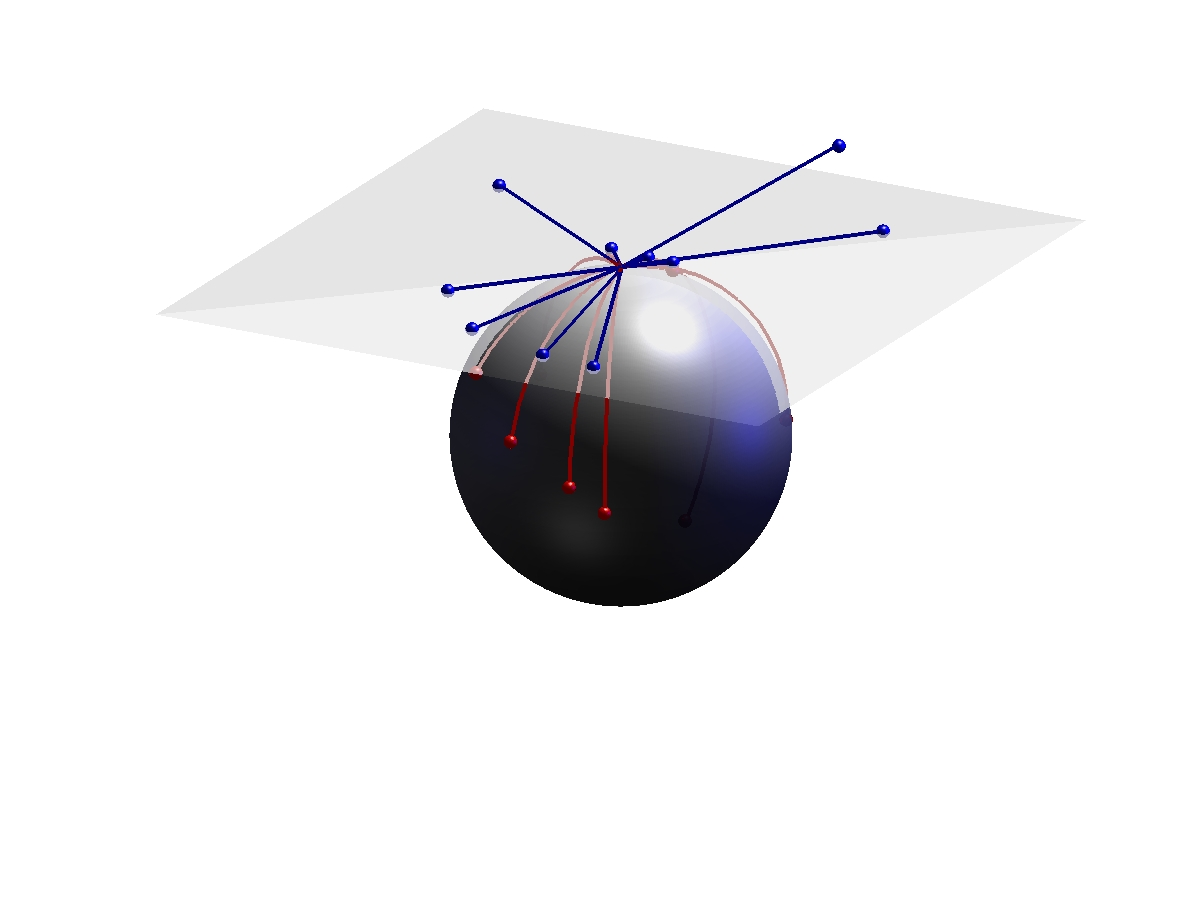
\includegraphics[width=\textwidth]{spheres}
\end{center}
%\end{columns}
\end{frame}

\begin{frame}
\frametitle{Exponential map}
\begin{columns}[c]
\column{0.6\textwidth}
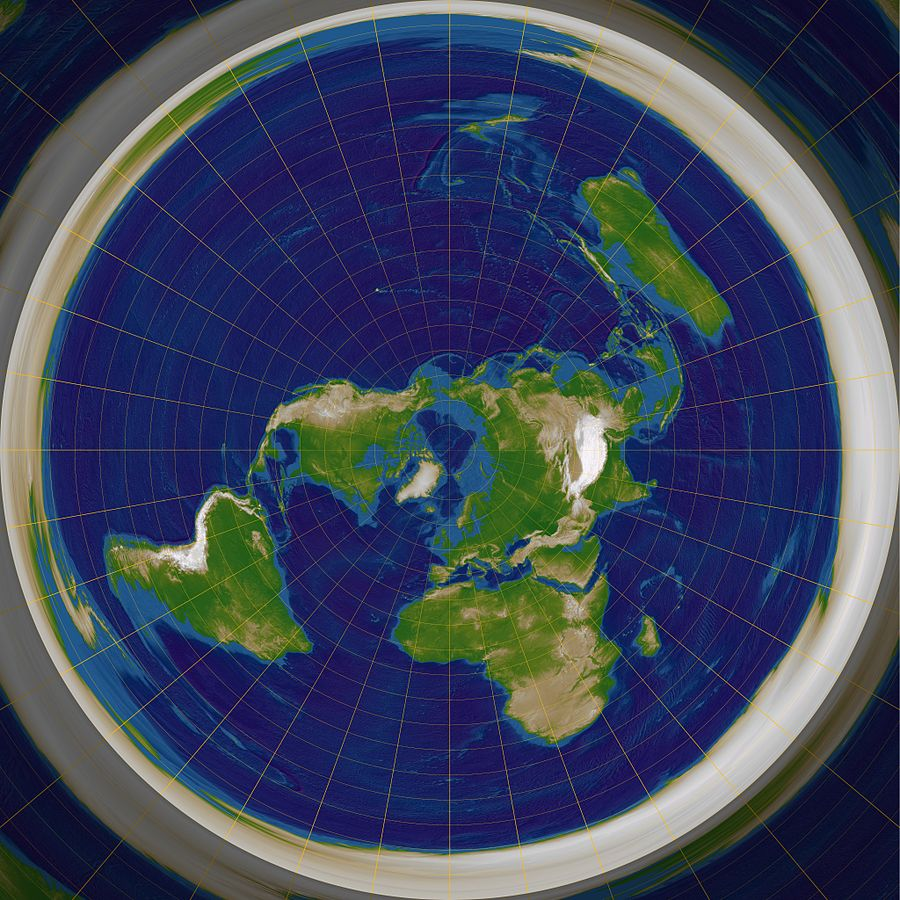
\includegraphics[width=\textwidth]{900px-Azimuthal_Equidistant_N90}
\column{0.4\textwidth}
\begin{center}
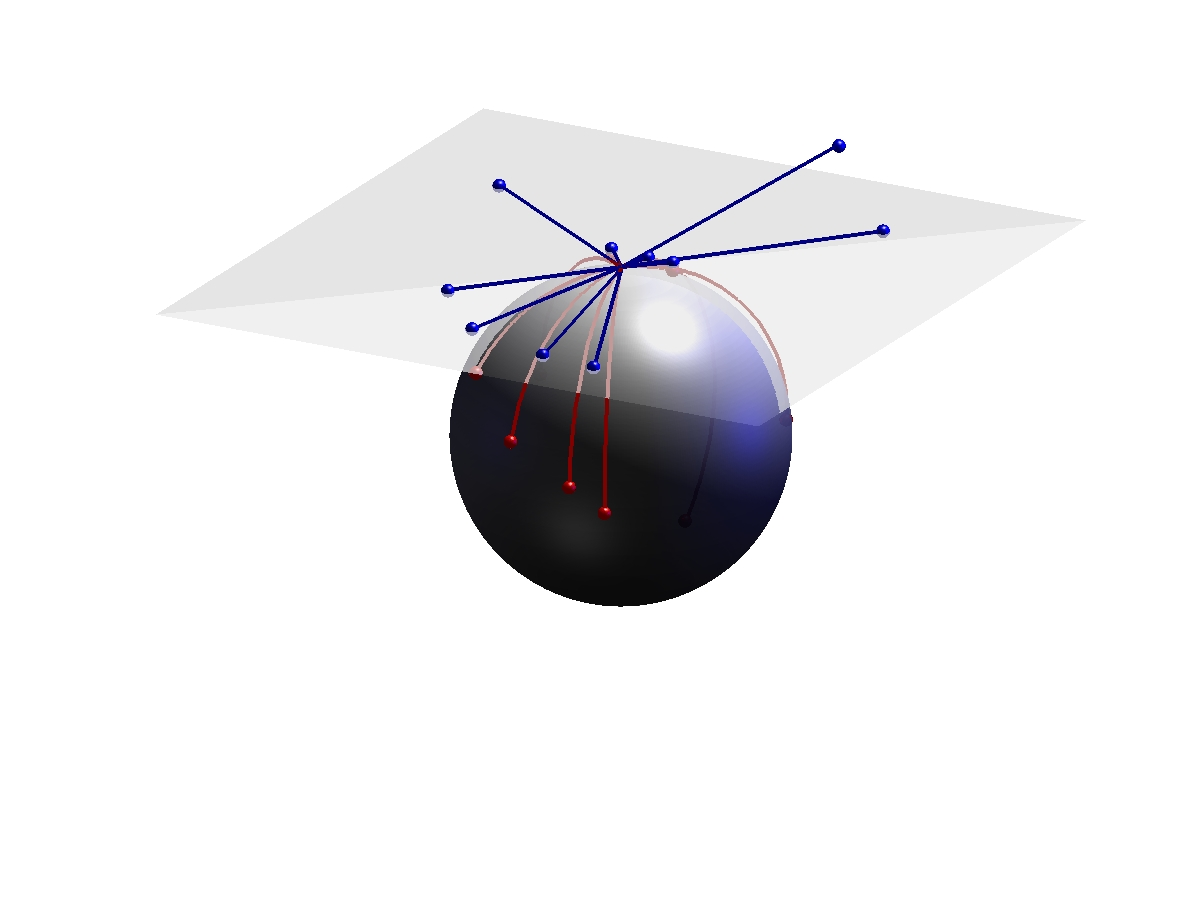
\includegraphics[width=\textwidth]{spheres}
\end{center}
\begin{tiny}
``Azimuthal Equidistant N90'' by RokerHRO - Own work. Licensed under CC BY-SA 3.0 via Wikimedia Commons - \url{http://commons.wikimedia.org/wiki/File:Azimuthal\_Equidistant\_N90.jpg}\par
\end{tiny}
\end{columns}
\end{frame}

\begin{frame}
\frametitle{LDDMM via ``geodesic shooting''}
\begin{columns}[c]
\column{0.65\textwidth}
In practice, we just need to estimate an initial velocity (${\bf v}_0$), from which we compute the initial momentum by ${\bf u}_0 = {\bf L}^{\dagger}{\bf L}{\bf v}_0$.

We set the deformation at time 0 to an identity transform (${\boldsymbol\varphi}_0 = Id$), and then evolve the following dynamical system for unit time:
\begin{eqnarray*}
{\bf u}_{t} = & \det |{\bf D}{\boldsymbol\varphi}_{t}^{-1}| ({\bf D}{\boldsymbol\varphi}_{t}^{-1})^T ({\bf u}_{0} \circ {\boldsymbol\varphi}_{t}^{-1})\cr
{\bf v}_{t} = & \left({\bf L}^{\dagger}{\bf L}\right)^{-1} {\bf u}_t\cr
\frac{d {\boldsymbol\varphi}}{d t} = & {\bf v}_t ({\boldsymbol\varphi}_t)
\end{eqnarray*}
\column{0.35\textwidth}
\begin{center}
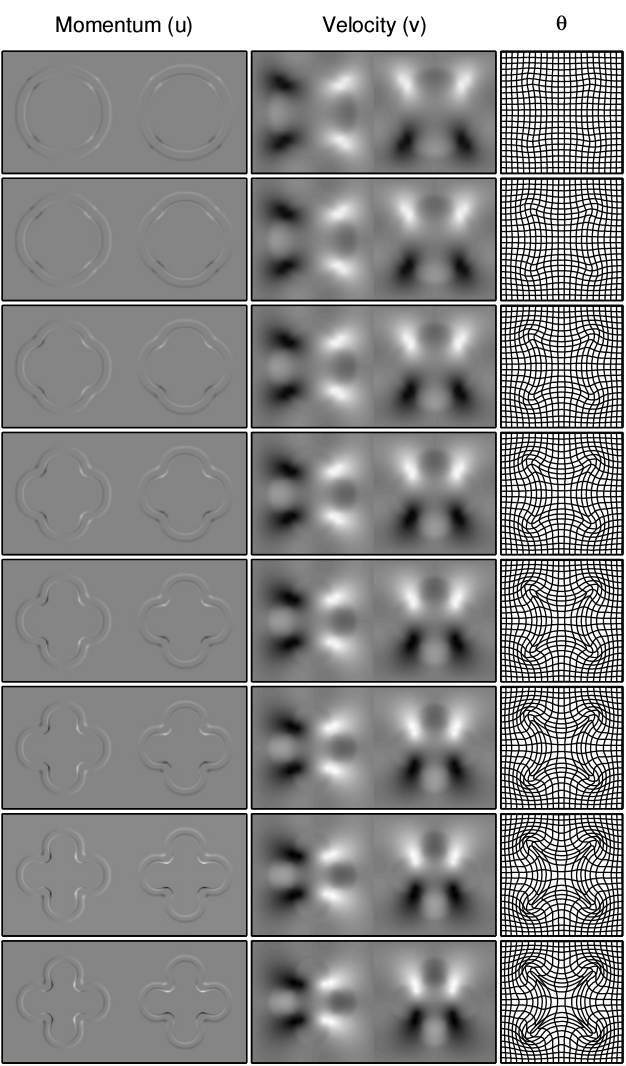
\includegraphics[width=1\textwidth]{evolution1}
\end{center}
\end{columns}
\vspace{.25cm}
\begin{tiny}
Younes, L, Arrate, F \& Miller, MI. \emph{Evolutions equations in computational anatomy}. Neuroimage 45(1S1):40--50 (2009).\par
\end{tiny}
\end{frame}


\begin{frame}
\frametitle{LDDMM via ``geodesic shooting''}
\begin{columns}[c]
\column{0.65\textwidth}
The final deformation (${\boldsymbol\varphi}_1$) is a type of exponential of the initial velocity (${\bf v}_0$).
\vspace{0.25cm}
\begin{tiny}
Exponential map (Riemannian geometry). (2015, January 13). In Wikipedia, The Free Encyclopedia. Retrieved 18:04, March 31, 2015, from \url{http://en.wikipedia.org/w/index.php?title=Exponential\_map\_(Riemannian\_geometry)\&oldid=642372186}\par
\end{tiny}
\column{0.35\textwidth}
\begin{center}
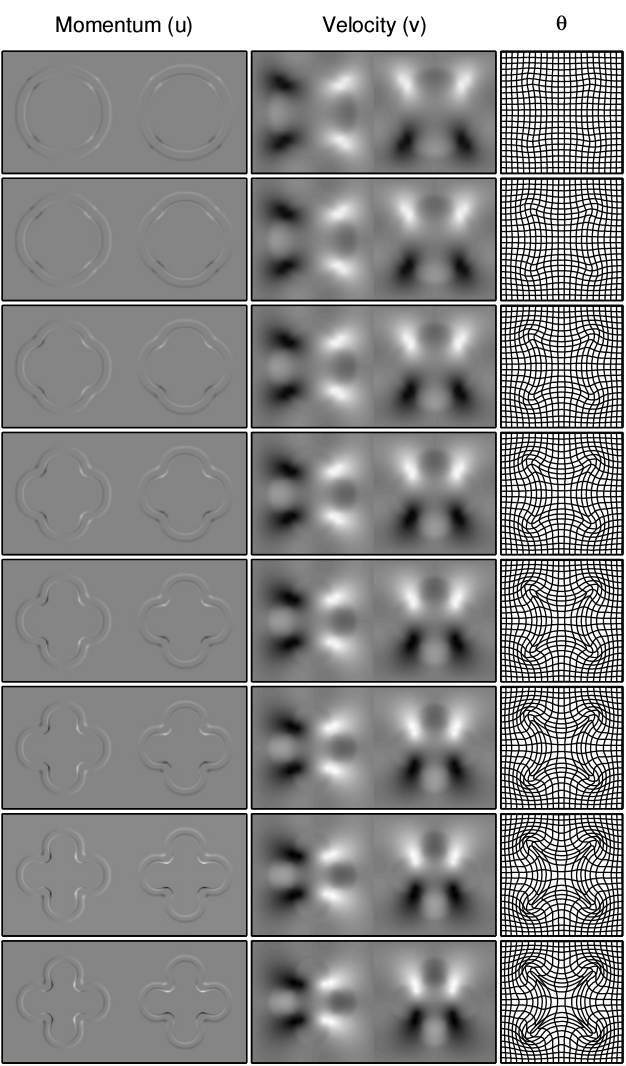
\includegraphics[width=1\textwidth]{evolution1}
\end{center}
\end{columns}

\vspace{.25cm}
\begin{tiny}
Younes, L, Arrate, F \& Miller, MI. \emph{Evolutions equations in computational anatomy}. Neuroimage 45(1S1):40--50 (2009).\par
\end{tiny}
\end{frame}


%%%%%%%%%%%%%%%%%%%%%%%%%%%%%%%%%%%%%%%%%%%%%%%%%%%%%%%%%%%%%%%

\begin{frame}
\frametitle{``Groupwise registration''}
Minimising distortions by centering around the mean.
\begin{center}
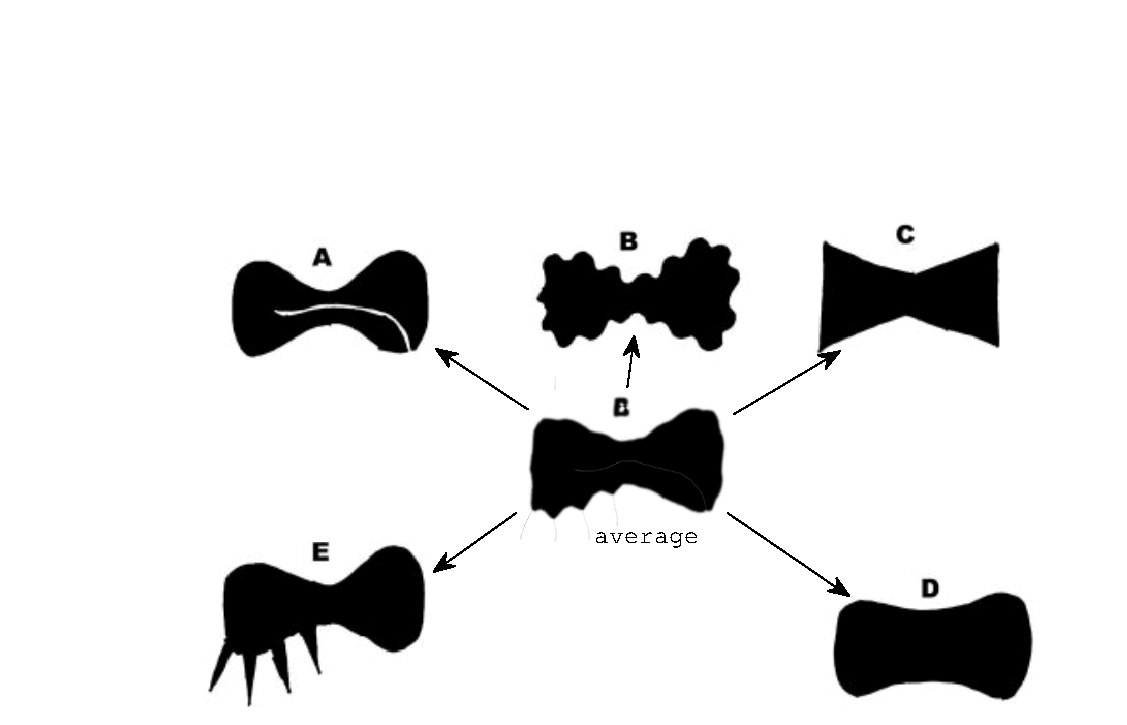
\includegraphics[width=.8\textwidth]{groupwise}
\end{center}
\end{frame}

\begin{frame}
\frametitle{``Groupwise registration''}
\begin{center}
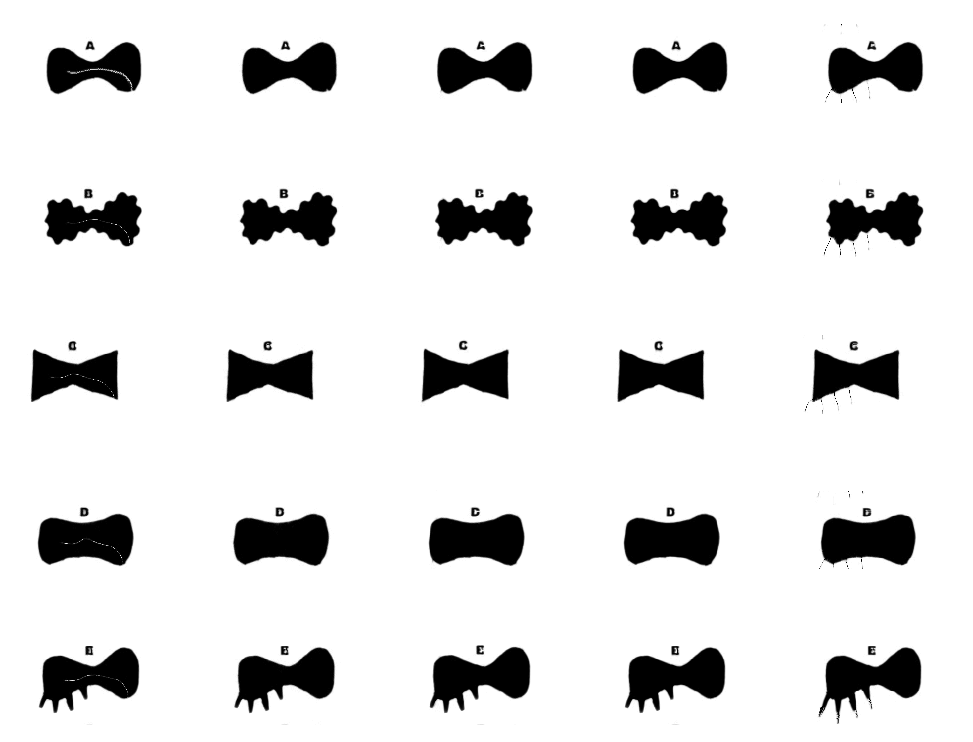
\includegraphics[width=.7\textwidth]{aligned_ties}
\end{center}
\end{frame}

\begin{frame}
\frametitle{``Groupwise registration''}
\begin{columns}[c]
\column{0.3\textwidth}
Ignoring the many technical details, the procedure involves alternating between:
\begin{itemize}
\item Create the mean of aligned images.
\item Align all images to be slightly closer to the mean.
\end{itemize}
\column{0.7\textwidth}
\begin{center}
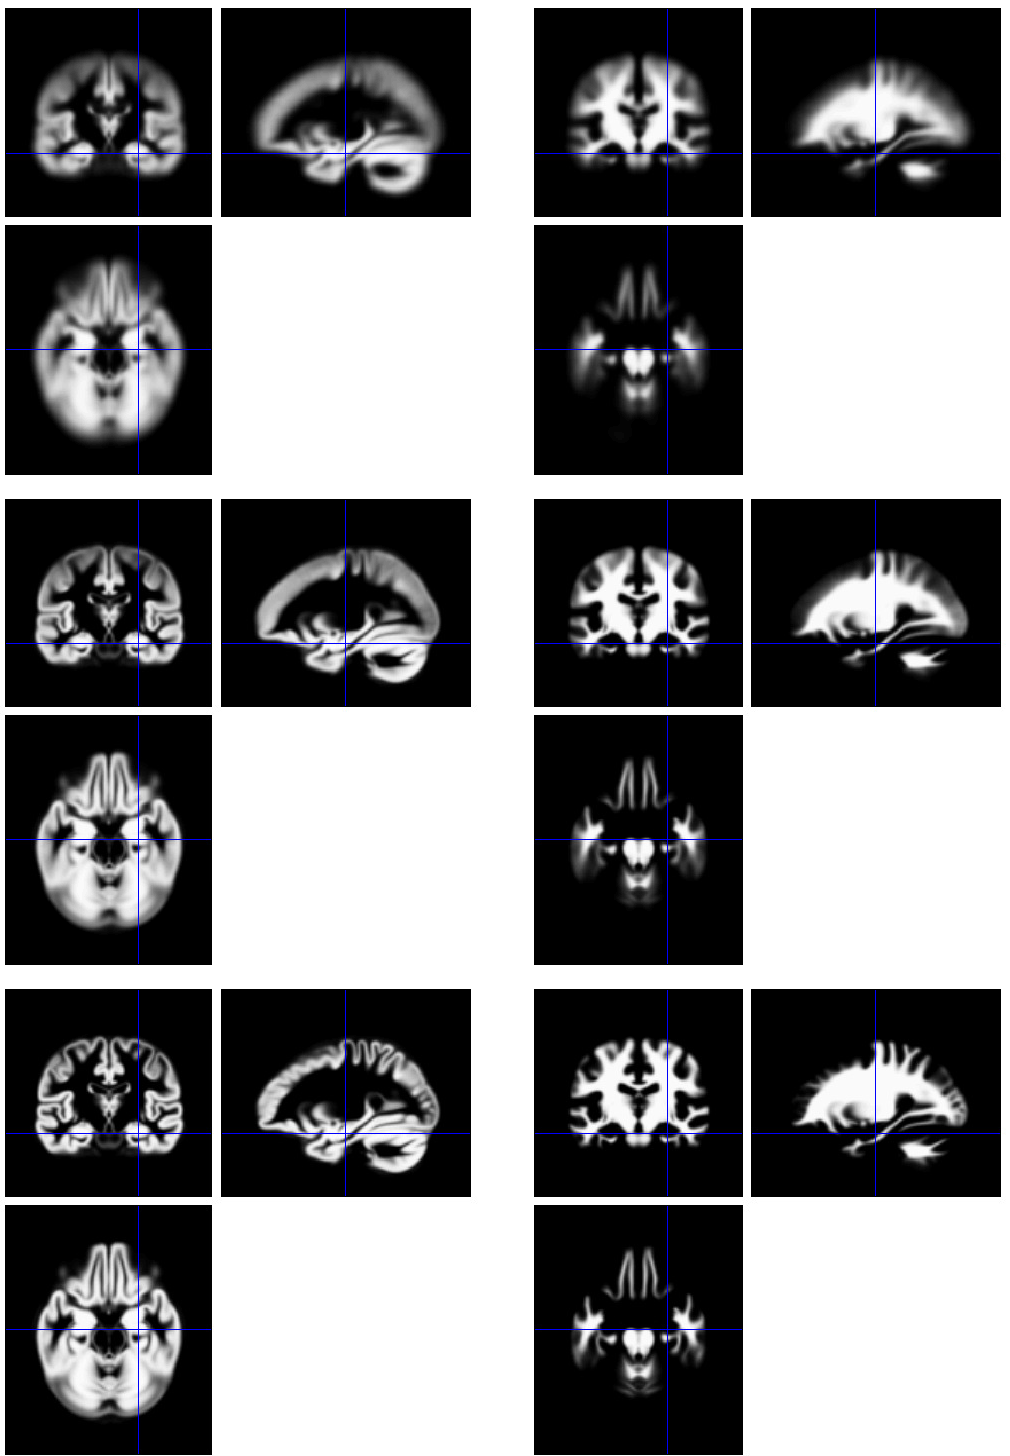
\includegraphics[height=.8\textheight]{groupwiseII}
\end{center}
\end{columns}
\end{frame}

\begin{frame}
\frametitle{Kernel matrix}
Construction of kernel matrix accounts for the regularisation used by the image registration:
\begin{Large}
\begin{align*}
k({\bf v},{\bf w}) & = \langle {\bf L}^{\dagger} {\bf L} {\bf v}, {\bf w} \rangle\cr
                   & = \langle {\bf L} {\bf v}, {\bf L} {\bf w} \rangle
\end{align*}
\end{Large}

\vspace{0.25cm}
\begin{tiny}
Wang, Lei, et al. ``Large deformation diffeomorphism and momentum based hippocampal shape discrimination in dementia of the Alzheimer type.'' Medical Imaging, IEEE Transactions on 26(4):462--470 (2007).\par
\end{tiny}
\end{frame}

%\begin{frame}
%\frametitle{D'Arcy Thompson's Generative Model}
%\begin{quote}
%``...diverse and dissimilar fishes can be referred as a whole to identical functions of very different co-ordinate systems...''
%\end{quote}
%\begin{center}
%
\includegraphics[height=0.4\textheight]{OGAF}
%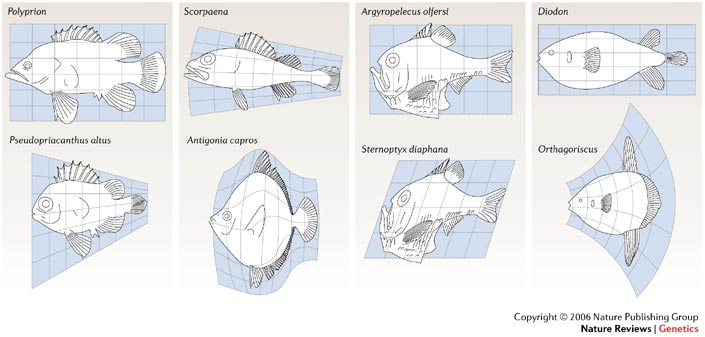
\includegraphics[height=0.4\textheight]{fish}
%\end{center}
%We can compute relative shapes using image registration.
%\end{frame}

% Top speed of an Airbus A380 is 1,020 km/h
% distance from NY:
% London 5576 km
% Los Angeles 3940 km

%\begin{frame}
%\frametitle{Kernel Matrices}
%Linear kernel matrices may computed from the raw features.
%\begin{eqnarray*}
%{\bf K} = {\bf X}{\bf X}^T
%\end{eqnarray*}
%A simple spatial feature selection may be considered as the following, where ${\bf W}$ is a diagonal matrix of ones and zeros:
%\begin{eqnarray*}
%{\bf K} = {\bf X}{\bf W}{\bf X}^T
%\end{eqnarray*}
%However, ${\bf W}$ may be more complicated, for example encoding spatial smoothing, high-pass filtering or any number of other things.
%\end{frame}

%\begin{frame}
%\frametitle{Inner Products}
%This gives us an alternative way of measuring distances between vectors in a linear way, where ${\bf W}$ is symmetric and positive definite.
%\begin{eqnarray*}
%d({\bf x}_1,{\bf x}_2) = \sqrt{({\bf x}_1 - {\bf x}_2)^T {\bf W} ({\bf x}_1 - {\bf x}_2)}
%\end{eqnarray*}
%
%Usually, the operation ${\bf W}{\bf x}^T$ is performed as a convolution.  For example, when dealing with 2D data, we may convolve with the Laplacian operator.
%\begin{eqnarray*}
%{\nabla}^2 {\bf x} = {\bf x} \ast \begin{pmatrix} 0 & -1 & 0\cr -1 & 4 & -1\cr 0 & -1 & 0\end{pmatrix}
%\end{eqnarray*}
%
%Note that the actual form of ${\bf W}$ can vary, so we need to figure out what metric tensor is optimal.
%\end{frame}

